\section{Introduction}
\label{sec:Int}
\subsection{Theme \& Topic Rationale}
\par This research focuses on the theme of Intelligent Transport Systems (ITS) and Autonomous Vehicle Sensor Perception. Getting an accurate estimate of a vehicle’s speed is super important for safety, especially for Advanced Driver Assistance Systems (ADAS) and autonomous navigation. While GPS is widely used, they frequently encounter signal degradation in urban canyons, tunnels, or adverse weather conditions, which can cause errors due to signal reflections (multipath errors) \cite{cui2003autonomous,li2025statistical}. On the other hand, estimating speed using dashcam footage is a cheaper, sensor-rich option \cite{pp2024video}, but it is inherently vulnerable to variations in lighting and computational latency. It’s important to compare these two methods against a highly accurate baseline, specifically vehicle CAN-bus data. Such comparison elucidates the specific environmental limitations of each system and offers empirical evidence to inform the development of improved algorithms in the future.
\subsection{Positioning \& Research Onion}
\par Based on Saunders’ Research Onion \cite{saunders2019research}, this research uses positivism, meaning seeing reality as something objective and separate from what other people think or interpret. The data that will be used is mainly measurable data like speeds, GPS coordinates and pixel shifts, with the researcher acting as an impartial observer by analysing the physical data. This research takes a deductive approach starting with already proved formulae and concepts such as the Haversine formula for GPS speeds and ego-motion tracking and comparing the data with each other to see which is more accurate. Even though the data comes from an archived source (Comma2k19) \cite{schafer2018commute}, the main objective for this research is to compare two algorithms under controlled conditions, using a steady CAN-bus ground truth to see how much error each algorithm has. Methodologically, the data is all quantitative because we are turning visual and geospatial information into numbers to analyse and compare statistically meaning there isn’t any qualitative data involved. The analysis is cross-sectional, so we are looking at a specific snapshot of data to test how well the algorithms work now, rather than tracking changes over time. Finally, we are collecting secondary data like video clips and GNSS logs to analyse and find the Mean Absolute Error for both algorithms.
\begin{figure}[htbp]
    \centering
    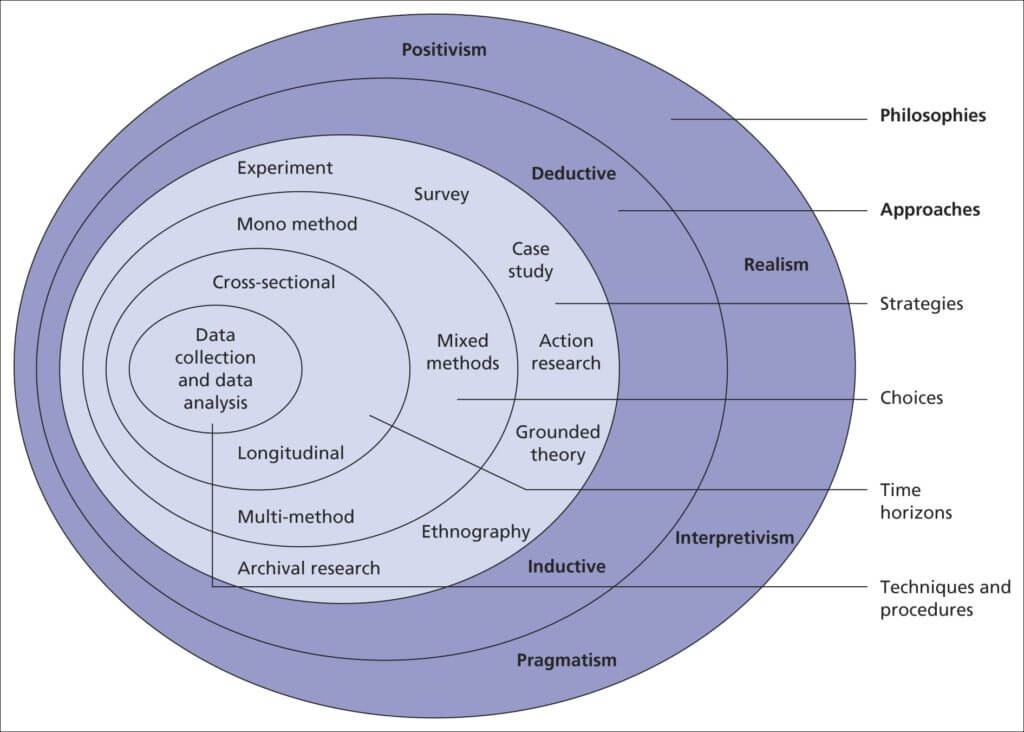
\includegraphics[scale=0.25]{includes/researchonion.jpg}
    \caption{Research Onion \cite{saunders2019research}}
    \label{fig:Onion}
\end{figure} 
\subsection{Background To This Research Theme}
\par The push towards fully autonomous vehicles has sped up the need for robust environmental awareness. In the past, navigation and speed checks have mostly relied on standard GPS receivers. But since self-driving technology needs accuracy to be down to milliseconds, the usual GPS signals and their delays or noise are not good enough \cite{cui2003autonomous}. Currently, recent advances in computer vision have made it possible to figure out “ego-motion”, basically how a camera moves through 3D space by tracking features \cite{pp2024video}. GPS can fail under bridges and cameras don’t work well in the dark or when there is lots of glare due to these drawbacks relying on just one sensor isn’t ideal thus the industry is leaning more towards combining different sensors. To manage to incorporate that well, researchers need to first understand how accurate each sensor is on its own and what kind of errors they might have when tested on real-world situations.
\subsection{Hypothesis}
\par This research works with a clear null hypothesis, which basically says there is no real difference in how accurate the vision-based algorithm is compared to GPS when it comes to estimating the vehicle’s true ground speed. On the other hand, the alternative hypothesis suggests that the vision-based method will have a smaller error margin than GPS during normal driving, mainly because commercial GPS units tend to have some delay and noise in their readings.
\subsection{Research Aim \& Purpose Statement}
\par The main goal of this study is to compare how accurately a vision-based speed estimation algorithm works versus a GPS-based one, using real-world dashcam footage. Ultimately, we are trying to spot the differences in how both methods measure speed. By testing against a solid ground truth, we hope to get useful insights into how reliable these sensors are, which could help in building safer autonomous vehicle navigation systems.
